\section{Примеры работы}

\subsection*{Пример 1}

Исходные данные:

\begin{lstlisting}
S O 3
S P 3
O Q 3
O P 2
P R 2
Q R 4
Q T 2
R T 3
\end{lstlisting}

Результат выполнения программы представлен на рис. \ref{fig:example_1}.

\begin{figure}[H]
    \centering
    
\includegraphics[width=\linewidth]{photo/example_1}
    \caption{Результ выполнения примера 1}
    \label{fig:example_1}
\end{figure}

Итоговый максимальный поток: 5

Результирующий граф представлен на рис. \ref{fig:example_graph_1}.

\begin{figure}[H]
    \centering
    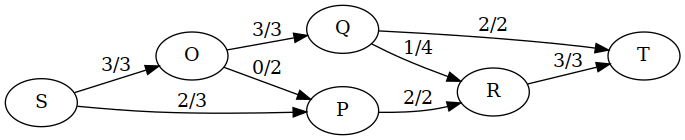
\includegraphics[width=\linewidth]{photo/example_graph_1}
    \caption{Результирующий граф для примера 1}
    \label{fig:example_graph_1}
\end{figure}

\subsection*{Пример 2}

Исходные данные:

\begin{lstlisting}
S A 8
S B 5
S C 3
A B 6
A C 4
A D 5
B C 5
B E 3
B F 5
C D 5
C E 4
D E 5
D T 3
E T 8
F E 3
F T 9
\end{lstlisting}

Результат выполнения программы представлен на рис. \ref{fig:example_2}.

\begin{figure}[H]
    \centering
    
\includegraphics[width=\linewidth]{photo/example_2}
    \caption{Результ выполнения примера 2}
    \label{fig:example_2}
\end{figure}

Итоговый максимальный поток: 16

Результирующий граф представлен на рис. \ref{fig:example_graph_2}.

\begin{figure}[H]
    \centering
    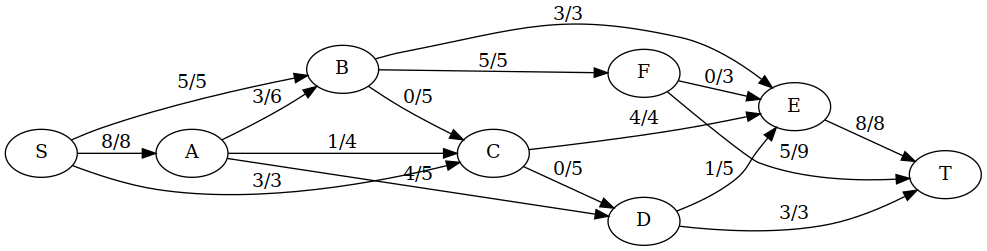
\includegraphics[width=\linewidth]{photo/example_graph_2}
    \caption{Результирующий граф для примера 2}
    \label{fig:example_graph_2}
\end{figure}

\subsection*{Пример 3}

Исходные данные:

\begin{lstlisting}
S A 5
S D 10
S G 5
A B 10
B C 10
B E 25
C T 5
D A 15
D E 20
E G 5
E F 30
F B 15
F T 15
F I 5
G H 5
H I 5
H F 5
I T 5
\end{lstlisting}

Результат выполнения программы представлен на рис. \ref{fig:example_3}.

\begin{figure}[H]
    \centering
    
\includegraphics[width=\linewidth]{photo/example_3}
    \caption{Результ выполнения примера 3}
    \label{fig:example_3}
\end{figure}

Итоговый максимальный поток: 20

Результирующий граф представлен на рис. \ref{fig:example_graph_3}.

\begin{figure}[H]
    \centering
    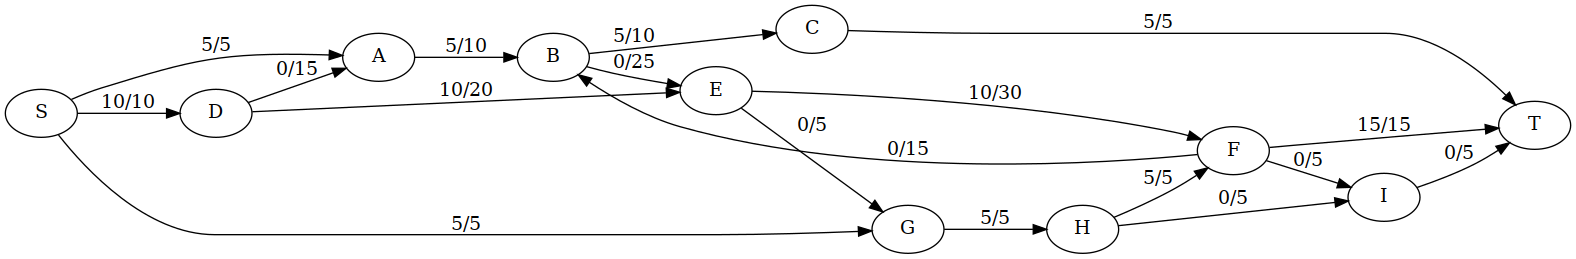
\includegraphics[width=\linewidth]{photo/example_graph_3}
    \caption{Результирующий граф для примера 3}
    \label{fig:example_graph_3}
\end{figure}

\subsection*{Пример 4}

Исходные данные:

\begin{lstlisting}
S A 8
S B 12
S C 26
S D 9
A E 3
B E 4
B F 6
C G 11
D G 2
D H 3
E I 9
E J 5
F J 7
G J 9
G K 2
H K 12
I T 8
J I 11
J K 20
K T 16
\end{lstlisting}

Результат выполнения программы представлен на рис. \ref{fig:example_4}.

\begin{figure}[H]
    \centering
    
\includegraphics[width=\linewidth]{photo/example_4}
    \caption{Результ выполнения примера 4}
    \label{fig:example_4}
\end{figure}

Итоговый максимальный поток: 24

Результирующий граф представлен на рис. \ref{fig:example_graph_4}.

\begin{figure}[H]
    \centering
    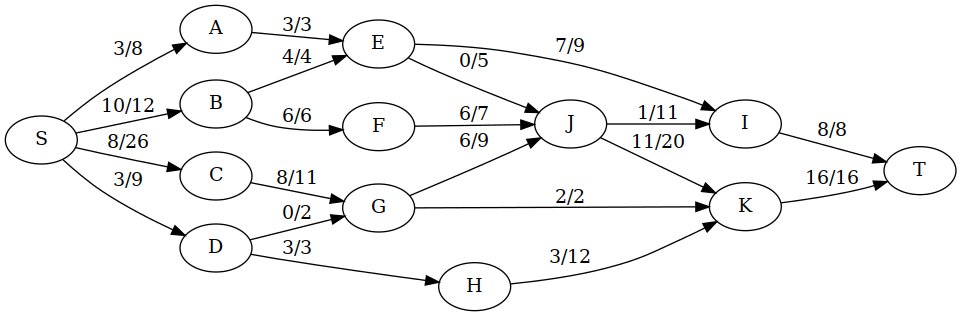
\includegraphics[width=\linewidth]{photo/example_graph_4}
    \caption{Результирующий граф для примера 4}
    \label{fig:example_graph_4}
\end{figure}

